\section{Transformers}
\label{appendix:transformers}

The transformer \cite{transformer}, built on self-attention (appendix \ref{appendix:attention}), is widely used in NLP tasks like translation, text generation, and classification. It consists of an encoder for input processing and a decoder for output generation, trained via maximum likelihood estimation (appendix \ref{appendix:likelihood_function}).

It is versatility in sequence-to-sequence tasks has expanded its applications to image and video synthesis models.





\subsection{Architecture}

\begin{figure}
    \centering
    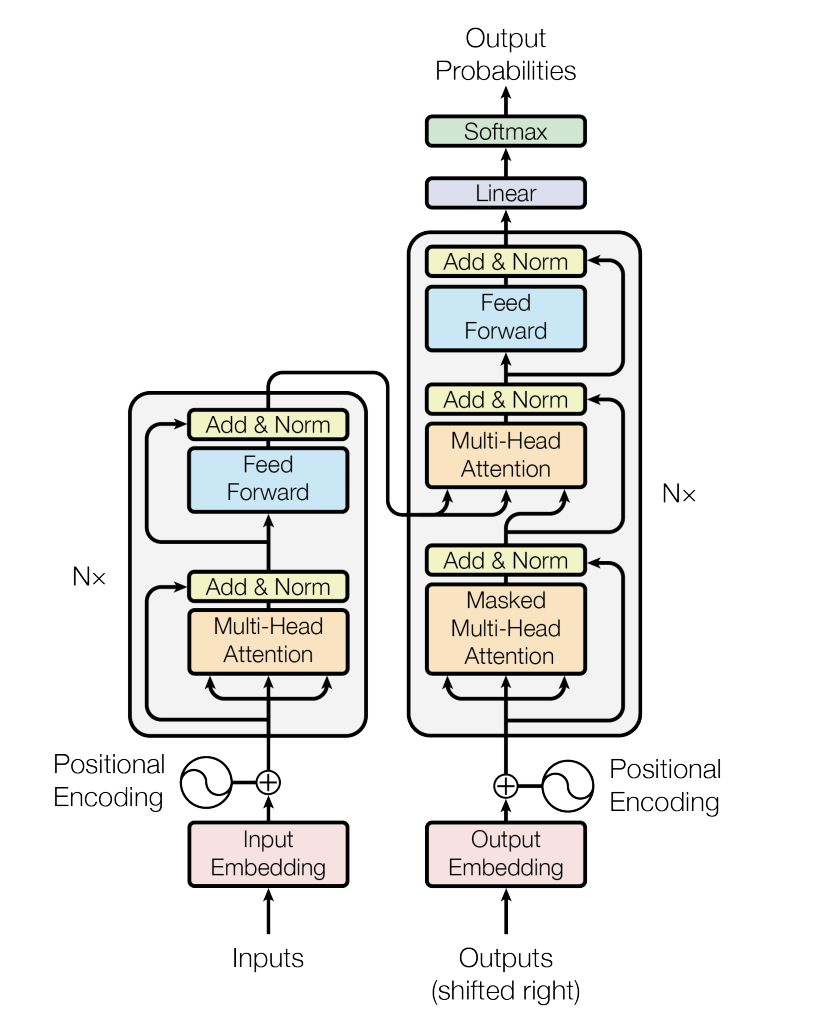
\includegraphics[width=0.4\textwidth]{images/appendix/transformer/architecture.png}
    \caption{Transformer architecture. The encoder (left) processes the input sequence, and the decoder (right) generates the output sequence \cite{transformer}.}
    \label{fig:appendix_transformer_architecture}
\end{figure}

The architecture overview is shown in figure \ref{fig:appendix_transformer_architecture}. The encoder processes the input sequence and breaks it down to meaningful representations, and the decoder takes these representations and generates output sequence in autoregressive fashion. 








\subsection*{Encoder}

The encoder processes a sequence of tokens, converted from text by a tokenizer (e.g., BERT, T5). Tokens are mapped to fixed-size vector embeddings through an embedding layer.

\textbf{Positional embeddings}: Since the transformer has no inherent understanding of sequence or order, positional encodings are added to each embedding to provide information about the position of each token in the sequence. Positional embeddings are added to token embeddings (figure \ref{fig:appendix_transformer_architecture}). The positional embeddings are computed as sinusoidal embeddings, (section \ref{subsec:sinusoidal_embeddings}).

\textbf{Multi-head attention}: Each encoder layer uses self-attention and feed-forward networks. Multi-head attention derives Q, K, and V matrices from the same input, unlike cross-attention.

\textbf{Add \& Norm}: Residual connections add the input to each layer's output, followed by layer normalization. This stabilizes training and helps to mitigate the exploding/vanishing gradient problem.









\subsection*{Decoder}

\textbf{Output embeddings}: Similar to input embeddings but shifted to the right in the input sequence, enabling the autoregressive generation of tokens. Positional embeddings are added, like in the encoder.

\textbf{Masked multi-head attention}: Prevents the model from attending to future tokens by masking, ensuring each token only considers itself and previous tokens.

\textbf{Multi-head cross-attention}: Allows the decoder to attend to encoder outputs (which is projected as K, V) and its previous layer outputs (projected as Q), enabling interaction between input and output sequences. Sometimes it is called "Encoder-Decoder Attention".

\textbf{Linear \& Softmax}: The decoder output passes through a linear layer and softmax to produce a probability distribution over the words' vocabulary. The most probable token is selected and fed back for the next step. In more advanced models, the output sometimes is not the most probable to allow more creative outputs. This is controlled by a 'temperature' parameter in the softmax function.

